\section{\MakeUppercase{System Architecture and Methodology}}
This section provides an overview of the system architecture and the methodology used in video \gls{codec} with a implicit neural network-based approach.
    \subsection{Block Diagram}
        \begin{figure}[H]
            \centering
            \includegraphics[width=\linewidth]{assets/Major Block Diagram.png}
            \caption{System Block Diagram}
            \label{fig:Block-Diagram}
        \end{figure}
        
        The block diagram outlines a comprehensive workflow for transmitting and receiving a video with audio through a compression and decompression pipeline. The process begins with the input video that includes both video and audio streams. In the transmitting end, the pre-processing pipeline separates the audio and video streams, downsampling the video to an NxM resolution and sampling the audio to match this resolution in terms of frequency. The extracted pixel values from the video are aligned with repeated audio samples to match the number of pixels, followed by normalization of pixel coordinates (x, y), the frame index (t), and the audio time step (T). The space-time coordinates (x, y, t) are then overfitted using Implicit Neural Representations (INR), preparing the data for compression. The compression pipeline applies knowledge distillation to simplify the model, followed by quantization to reduce data precision and encoding for efficient transmission. The compressed model is then transmitted through a guided or unguided channel. On the receiving end, the compressed model undergoes a decompression pipeline that includes decoding and dequantization to restore the original scale of the data. The post-processing pipeline processes the RGB pixel output along with derived amplitude values per pixel, which are used to reconstruct the video and audio. Finally, the output is the reconstructed video with audio, ensuring the transmitted data is efficiently compressed and accurately restored at the receiving end.

        \subsubsection{Input Video with Audio}
        The process begins with an input video that includes both visual and auditory information, serving as the source material for the subsequent encoding and compression processes.

        \subsubsection{Pre-processing Pipeline}
        \begin{figure}[H]
            \centering
            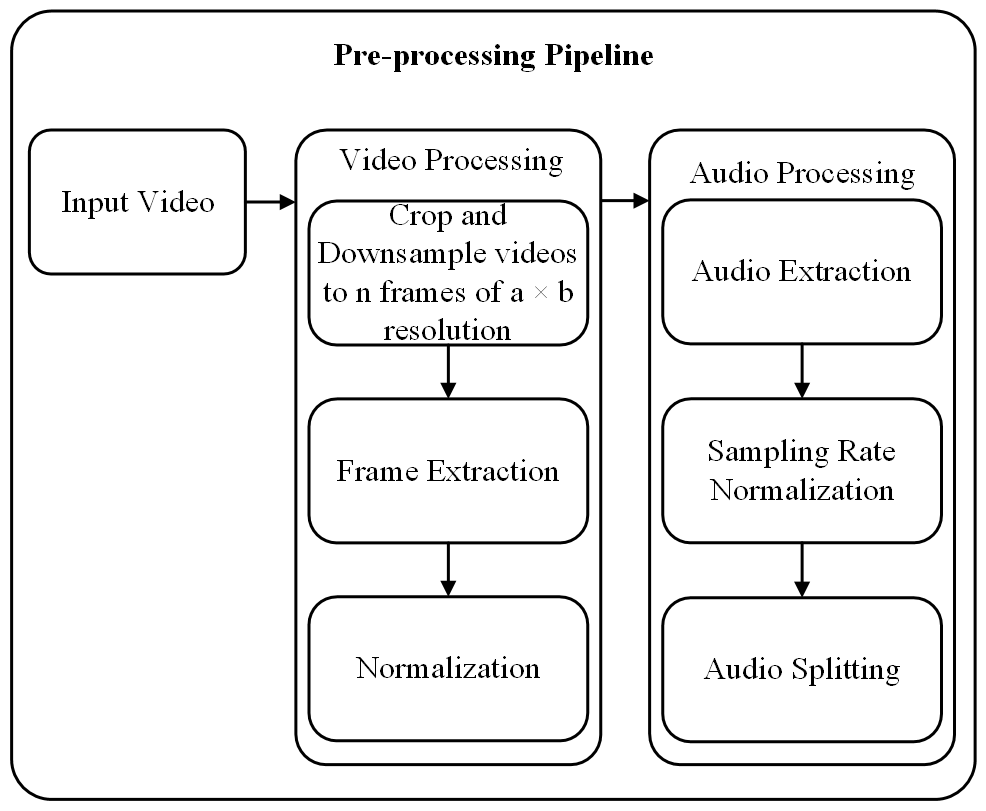
\includegraphics[width=0.9\linewidth]{assets/Major Data Pre-Processing.png}
            \caption{Pre-processing Pipeline}
            \label{fig:pre-processing-pipeline}
        \end{figure}
        
        \textbf{Overview of the Pre-processing Pipeline for Video with Audio}
        The figure illustrates a pre-processing pipeline designed for handling video files with accompanying audio tracks. The pipeline is organized into two main branches: one for processing video data and the other for audio data. Each branch standardizes and optimizes the respective data types, ensuring compatibility for integration and further analysis or processing.
        
        \textbf{Video Processing Branch}
        \begin{itemize}
            \item \textbf{Crop and Downsample Videos to \(n\) Frames of \(a \times b\) Resolution:} 
            Video frames are cropped and resized to a fixed resolution of \(a \times b\). This step reduces the complexity of the video data, making it computationally efficient while preserving essential visual information. Additionally, the video is downsampled to \(n\) frames, ensuring a uniform frame rate and minimizing redundancy.
        
            \item \textbf{Pixel Extraction:} 
            After downsampling, individual pixel values are extracted from each video frame. These pixel values represent the visual content of the video and encapsulate the color and intensity information for each frame.
        
            \item \textbf{Normalization:} 
            The extracted pixel values are normalized to a standard range, typically between 0 and 1. Normalization ensures consistency in data representation, minimizes numerical instability, and facilitates improved performance in subsequent processing stages.
        \end{itemize}
        
        \textbf{Audio Processing Branch}
        \begin{itemize}
            \item \textbf{Audio Extraction at Sample Rate \(a \times b\) kHz:} 
            The audio data is extracted from the input video and resampled to match the video resolution, specifically at a sample rate proportional to the resolution (\(a \times b\) kHz). This alignment ensures that the audio data corresponds directly to the spatial dimensions of the video frames.
        
            \item \textbf{Sampling Rate Normalization:} 
            The resampled audio undergoes normalization to standardize its amplitude range. This ensures uniformity in the audio data and aligns it with the normalized video pixel data.
        
            \item \textbf{Repeat Audio to Match the Number of Pixels:} 
            To synchronize the audio with the video data, audio samples are repeated so that their quantity matches the number of pixels in each video frame. This step ensures compatibility between the audio and video data for seamless integration and processing.
        \end{itemize}
        
        After pre-processing, the video and audio data are standardized and aligned for integration. The video frames with normalized pixel data and the corresponding audio samples are represented in a unified format. This unified representation ensures that the input data is prepared and ready for further processing, including model fitting and analysis.
        
        \subsubsection{Training Model (Fully Connected Neural Network)}
        A specially designed neural network consisting of multiple fully connected layers is trained to accept space-time coordinates as input and output the corresponding \gls{rgb} values for pixels and the amplitude for the audio, effectively mapping these inputs to their visual and auditory outputs.
    
        \subsubsection{Compression Pipeline}
        \begin{enumerate}[label=\textbf{\roman*.}]
            \item \textbf{Knowledge Distillation:} A smaller model is trained to mimic the behavior of a larger overfitted model, effectively transferring knowledge while reducing the complexity of the model.
            \item \textbf{16-bit Integer Quantization:} The network parameters are reduced in precision by quantizing them to 16-bit integers, which decreases the model size while retaining essential information and minimizing performance loss.
            \item \textbf{Model Encoding:} The quantized model weights are encoded using \gls{lzma}. This process compresses the quantized weights into a compact and efficient representation for transmission or storage.
        \end{enumerate}
        \subsubsection{Transmission and Decompression}

        After the model has been processed through the compression pipeline, it is transmitted over a guided or unguided channel to the receiving end. This transmission ensures that the compressed and encoded model reaches its destination efficiently, preserving the integrity of the compressed data.

        Once received, the model undergoes a decompression process, starting with \textbf{decoding}. In this step, the encoded data is converted back into its quantized format. The decoding process reverses the arithmetic or range encoding applied during the compression pipeline in \gls{lzma}, ensuring that the quantized weights and parameters are accurately restored.

        Following decoding, the model is passed through \textbf{dequantization}. During this step, the quantized data, represented as 16-bit integers, is scaled back to its original precision range. This scaling is achieved using the quantization parameters (such as scale and zero-point) that were preserved during the compression process. Dequantization restores the numerical accuracy of the model while maintaining the reduced size achieved through quantization.

        The decompressed model, now in its restored form, is ready for inference. At this stage, it provides RGB values for each pixel and amplitude values for audio corresponding to the space-time coordinates $\left[(x, y, t), T\right]$. These outputs serve as the foundation for the subsequent steps in the post-processing pipeline.'

        \subsubsection{Post-processing Pipeline}
        \begin{figure}[H]
            \centering
            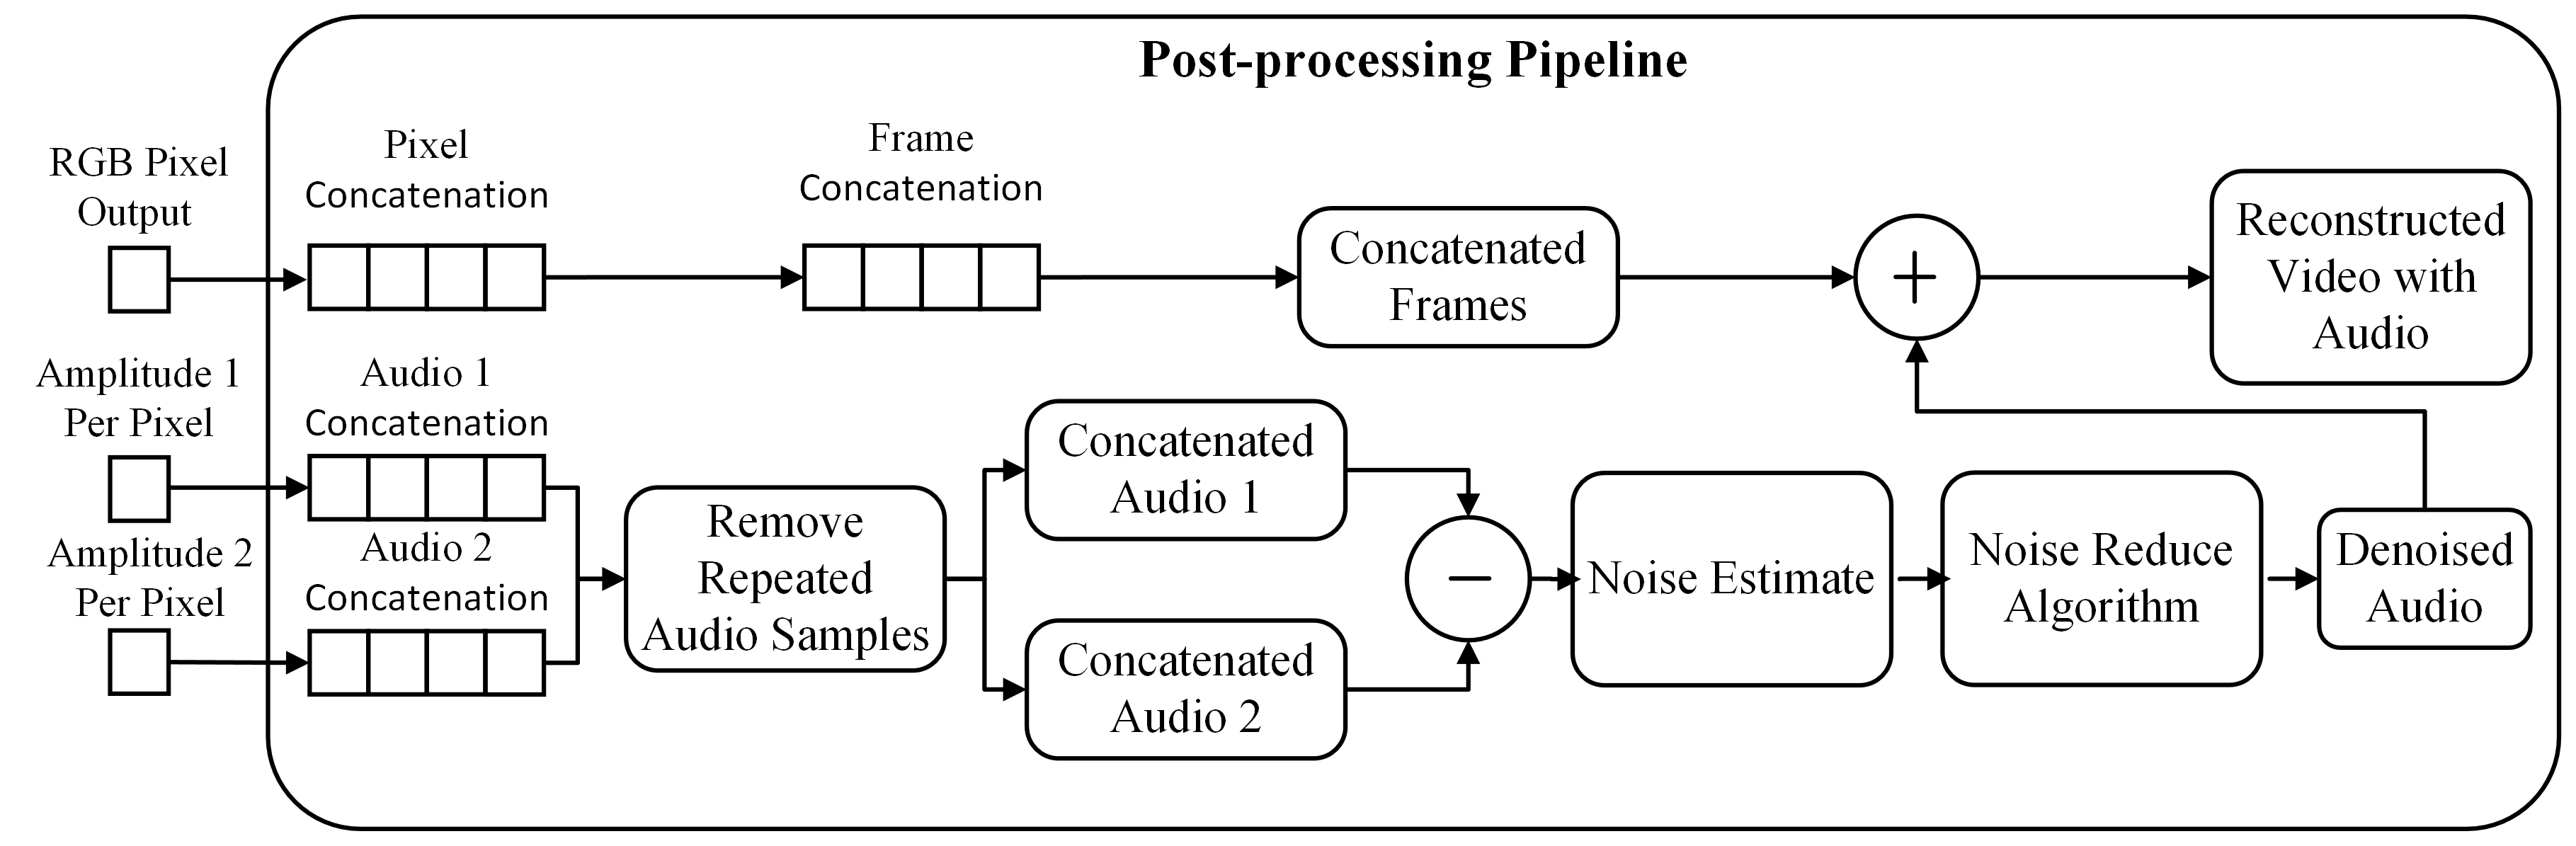
\includegraphics[width=0.9\linewidth]{assets/Major Data Post-Processing.png}
            \caption{Post-processing Pipeline}
            \label{fig:post-processing-pipeline}
        \end{figure}
        The post-processing pipeline illustrated in \autoref{fig:post-processing-pipeline} outlines the steps taken after the transmitted model has been decompressed and dequantized. The decompressed model is inferenced to retrieve the respective RGB values and audio amplitude values for the space-time coordinates $\left[(x, y, t), T\right]$. These outputs are critical for reconstructing the video and audio components.

        The RGB values for each pixel are extracted and concatenated into a tensor that represents the color information for the video frames. Similarly, the model outputs two amplitude values for the audio—Amplitude 1 and Amplitude 2—corresponding to each pixel. These amplitude values are concatenated to form a unified audio signal. However, the concatenated audio includes repeated samples, which are removed in the next step to match the original audio sample rate and timing. This ensures the audio remains synchronized with the video frames.
        
        To enhance the audio quality, a noise reduction process is performed. The two audio outputs (Concatenated Audio 1 and Concatenated Audio 2) are subtracted to estimate the noise present in the audio. The estimated noise, along with one of the audio outputs, is then passed through a noise reduction algorithm. This algorithm processes the signals to produce a denoised audio output that is free from distortions and artifacts.
        
        Meanwhile, the concatenated RGB values are used to generate individual video frames. These frames are then merged to reconstruct the full video. Finally, the denoised audio is combined with the reconstructed video to create the complete decompressed video with synchronized audio. This pipeline ensures a high-quality output with minimal noise and distortion, preserving the fidelity of the original input.
    \subsubsection{Noise Reduction Process}
    During the training and inference phases, the generated audio signals contained residual noise, which was due to imperfections in the model's processing. To address this, we applied a noise reduction algorithm specifically designed to suppress this residual noise while preserving the integrity of the audio content. The noise estimate was obtained by leveraging the two audio output branches, which generated two inferred outputs for the same signal; the difference between these outputs was used to estimate the noise. Using this noise estimate, a dedicated noise clip was extracted to compute noise characteristics such as mean and standard deviation across frequency bands. A dynamic noise threshold was then determined and applied to the audio spectrogram, followed by Gaussian smoothing to refine the noise suppression mask. This process effectively removed the residual noise and ensured the reconstructed audio maintained high fidelity.
    The following section details the implementation of this noise reduction algorithm.
    \begin{algorithm}[H]
        \caption{Noise Reduction Algorithm}
        \label{alg:noise_reduction}
        \begin{algorithmic}[1]
        \REQUIRE audio\_clip, noise\_clip, parameters (smoothing parameters, FFT size, and threshold control)
        
        \STATE \textbf{Compute Spectrogram of Noise:}
        \STATE noise\_stft $\gets$ \texttt{STFT(noise\_clip)}
        \STATE noise\_stft\_db $\gets$ \texttt{ConvertToDB(noise\_stft)}
        \STATE mean\_freq\_noise $\gets$ \texttt{Mean(noise\_stft\_db, axis=freq)}
        \STATE std\_freq\_noise $\gets$ \texttt{Std(noise\_stft\_db, axis=freq)}
        \STATE noise\_threshold $\gets$ mean\_freq\_noise + $k \times$ std\_freq\_noise
        
        \STATE \textbf{Compute Spectrogram of Audio:}
        \STATE sig\_stft $\gets$ \texttt{STFT(audio\_clip)}
        \STATE sig\_stft\_db $\gets$ \texttt{ConvertToDB(sig\_stft)}
        
        \STATE \textbf{Generate Mask:}
        \STATE sig\_mask $\gets$ (sig\_stft\_db $>$ noise\_threshold)
        \STATE smoothed\_mask $\gets$ \texttt{ApplyGaussianFilter(sig\_mask)}
        
        \STATE \textbf{Apply Mask:}
        \STATE masked\_stft $\gets$ sig\_stft $\times$ smoothed\_mask
        
        \STATE \textbf{Reconstruct Signal:}
        \STATE recovered\_signal $\gets$ \texttt{ISTFT(masked\_stft)}
        
        \RETURN recovered\_signal
        \end{algorithmic}
    \end{algorithm}
    
    \subsection{Quantization}
    \textit{Quantization} in machine learning is the process of reducing the number of bits that represent the model's weights and activations. It typically involves converting 32-bit floating-point numbers to lower precision formats like 16-bit, 8-bit, or even binary (1-bit) representations. This reduces the model size and accelerates inference on hardware with limited computational resources.

    \autoref{alg:model-quantization} outline the process of model quantization, which aims to reduce the precision of neural network weights to improve efficiency. The process begins with a trained neural network model. The first step is to choose a quantization scheme, which can be either uniform quantization, where weights are mapped to fixed, uniformly distributed levels, or non-uniform quantization, where techniques like k-means clustering are used to determine the mapping. Following this, the number of quantization levels $Q$ is determined (e.g., 8-bit, 16-bit). Each weight $W_{ij}$ in the model is then mapped to the nearest quantization level within $Q$. The original weights $W$ are replaced with these quantized weights, resulting in a quantized model. Optionally, the quantized model can be fine-tuned on the training dataset to recover any lost accuracy. The final step is to return the quantized model $Q(W)$. This approach effectively reduces the model's memory footprint and potentially improves its computational efficiency while maintaining its performance.
    
    \begin{algorithm}[H]
        \caption{Model Quantization}
        \label{alg:model-quantization}
        \begin{algorithmic}[1]
        \REQUIRE Neural network model with weights $W$, training dataset, quantization levels $Q$ (e.g., 8-bit, 16-bit)
        
        \STATE Train the model on the training dataset
        \STATE Find zero-point and scale factor for each layer
        \FOR{each weight $W_{ij}$ in $W$}
            \STATE Map $W_{ij}$ to the nearest quantization level in $Q$
        \ENDFOR
        \STATE Replace original weights $W$ with quantized weights $Q(W)$
        \STATE Also store the scale factor and zero-point for each layer
        
        \RETURN $Q(W)$
        \end{algorithmic}
    \end{algorithm}
        

    \subsection{Loss Function}
    To effectively generate \gls{inr} for audio-video data, it is essential to define appropriate loss functions that guide the learning process. Below, the specific loss functions for audio and video are introduced, followed by the formulation of a combined loss function that integrates both modalities.

        \subsubsection{Audio Loss Function}
        The loss function for audio data is defined as:
        \begin{equation}
            \mathcal{L}_{\text{audio}} = 0.5 \left( \int_{\Omega_{\text{audio}}} \| \Phi_{\text{audio,1}}(t) - f_{\text{audio}}(t) \| \, dt \right) + 0.5 \left( \int_{\Omega_{\text{audio}}} \| \Phi_{\text{audio,2}}(t) - f_{\text{audio}}(t) \| \, dt \right)
        \end{equation}
        where,
        \begin{itemize}
            \item \( t \in \mathbb{R} \) is the time point,
            \item  \( \Phi_{\text{audio,1}}(t) \) is the first audio output of the model at time \( t \),
            \item \( \Phi_{\text{audio,2}}(t) \) is the second audio output of the model at time \( t \),
            \item \( f_{\text{audio}}(t) \) is the ground truth audio amplitude at time \( t \),
            \item \( \Omega_{\text{audio}} \) is the time interval over which the audio is defined.
        \end{itemize}
    
        \subsubsection{Video Loss Function}
            The loss function for video data is defined as:
        \begin{equation}
            \mathcal{L}_{\text{video}} = \int_{\Omega_{\text{video}}} \| \Phi_{\text{video}}(x, t) - f_{\text{video}}(x, t) \| \, dx \, dt
        \end{equation}
        where,
        \begin{itemize}
        \item \( (x, t) \in \mathbb{R}^3 \) represents the space-time coordinates,
        \item \( \Phi_{\text{video}}(x, t) \) is the model's output for the video at space-time coordinate \( (x, t) \),
        \item \( f_{\text{video}}(x, t) \) is the ground truth RGB value at space-time coordinate \( (x, t) \),
        \item \( \Omega_{\text{video}} \) is the space-time region over which the video is defined.
        \end{itemize}
    
        \subsubsection{Combined Teacher Loss Function}
        The combined loss function for both audio and video data is formulated as:
        \begin{equation}
            \mathcal{L}_{\text{combined}} = \lambda_{\text{audio}} \mathcal{L}_{\text{audio}} + \lambda_{\text{video}} \mathcal{L}_{\text{video}}
            \end{equation}
            where,
            \begin{itemize}
                \item \( \lambda_{\text{audio}} \) is the weight that balances the contribution of the audio loss,
                \item \( \lambda_{\text{video}} \) is the weight that balances the contribution of video loss.
            \end{itemize}
    This combined loss function ensures that both the audio and video outputs are supervised and optimized simultaneously.

    \subsubsection{Knowledge Distillation Loss Function}
    The Knowledge Distillation (KD) loss function is formulated to combine both the hard and soft loss components for audio and video data. The overall loss is defined as:

    \begin{equation}
        \mathcal{L}_{\text{KD}} = \alpha \mathcal{L}_{\text{hard}} + (1 - \alpha) \mathcal{L}_{\text{soft}}
    \end{equation}
    where,

    \begin{itemize}
        \item \( \alpha \) is a hyperparameter that balances the contribution of the hard and soft loss components,
        \item \( \mathcal{L}_{\text{hard}} \) is the total hard loss (based on the student's output and the ground truth),
        \item \( \mathcal{L}_{\text{soft}} \) is the total soft loss (based on the student's output and the teacher's output).
    \end{itemize}

    The hard and soft losses are defined as:

    \begin{equation}
        \mathcal{L}_{\text{hard}} = 0.5 \times \mathcal{L}_{\text{video, hard}} + 0.5 \times \left( 0.5 \times \mathcal{L}_{\text{audio, hard}} + 0.5 \times \mathcal{L}_{\text{audio(siam), hard}} \right)
    \end{equation}

    \begin{equation}
        \mathcal{L}_{\text{soft}} = 0.5 \times \mathcal{L}_{\text{video, soft}} + 0.5 \times \left( 0.5 \times \mathcal{L}_{\text{audio, soft}} + 0.5 \times \mathcal{L}_{\text{audio(siam), soft}} \right)
    \end{equation}

    
    \subsection{Evaluation Metrics for Video}
        To rigorously evaluate the effectiveness of our proposed INR based video compression technique, we will utilize a suite of metrics that assess various dimensions of video quality, including visual fidelity, perceptual quality, and predictive accuracy. Here's an overview of each metric, their numerical value ranges, and whether it's preferable for their values to increase or decrease:
        \subsubsection{Peak Signal-to-Noise Ratio}
            \begin{itemize}
                \item \textbf{Overview}: \gls{psnr} is commonly employed to measure the quality of reconstruction in lossy compression \gls{codec}s. It compares the similarity between the original and compressed video by measuring the ratio between the maximum possible power of a signal and the power of distorting noise.
                \item \textbf{Value Range}: Typically expressed in \gls{db}, the higher the \gls{psnr}, the better the quality of the compressed video. A higher \gls{psnr} value indicates that the reconstruction is of higher quality.
                \item \textbf{Preference} $\uparrow$: Values typically range from 20 to 50 \gls{db}, where higher values (around 40 \gls{db} or more) represent excellent quality.
                \item \textbf{Formula}
                \begin{equation}\label{eqn:PSNR}
                    \text{PSNR} = 20 \cdot \log_{10}\left(\frac{{\text{MAX}_I}}{\sqrt{\text{MSE}}}\right)
                \end{equation}
                where, $\text{MAX}_I$ is the maximum possible pixel value of the image (e.g., 255 for 8-bit images), and $\text{MSE}$ is the mean squared error between the original and compressed image.
               \end{itemize} 

        \subsubsection{Signal-to-Quantization Noise Ratio (SQNR)}
        \label{subsubsec:SQNR}
        \begin{itemize}
            \item \textbf{Overview}: \gls{sqnr} is a widely used metric to assess the quality of quantized signals in digital signal processing and machine learning models. It measures the ratio of the power of the original signal to the power of the noise introduced during quantization.
            \item \textbf{Value Range}: Typically expressed in \gls{db}, higher \gls{sqnr} values indicate better fidelity of the quantized signal to the original. A perfect quantization would result in an infinite \gls{sqnr}.
            \item \textbf{Preference} $\uparrow$: Higher values are preferred, as they represent lower quantization noise. For practical systems, values depend on the bit depth and dynamic range of the quantizer.
            \item \textbf{Formula}
            \begin{equation}\label{eqn:SQNR}
                \text{SQNR} = 10 \cdot \log_{10}\left(\frac{P_s}{P_n}\right)
            \end{equation}
            where, \(P_s\) is the signal power, defined as:
            \begin{equation}
                P_s = \frac{1}{N} \sum_{i=1}^N x_i^2
            \end{equation}
            and \(P_n\) is the quantization noise power, defined as:
            \begin{equation}
                P_n = \frac{1}{N} \sum_{i=1}^N (x_i - \hat{x}_i)^2
            \end{equation}
            Here, \(x_i\) is the original signal, \(\hat{x}_i\) is the quantized signal, and \(N\) is the number of samples.
        \end{itemize}
               
           
        \subsubsection{Learned Perceptual Image Patch Similarity}
            \begin{itemize}
                \item \textbf{Overview}: \gls{lpips} metric evaluates the perceptual difference between two images or videos. Unlike traditional metrics that focus on pixel-level accuracy, \gls{lpips} uses deep learning to assess how perceptually similar two images are to the human eye.
                \item \textbf{Value Range}: This metric produces a similarity score that ranges from 0 to 1, where lower scores indicate greater perceptual similarity.
                \item \textbf{Preference} $\downarrow$: A lower \gls{lpips} score means that the compressed video is perceptually closer to the original, indicating better compression performance.
            \end{itemize}

        \subsubsection{Structural Similarity Index Measure}
            \begin{itemize}
                \item \textbf{Overview}: \gls{ssim} is used to measure the similarity between two images or videos. It considers attributes that are important to the human visual system such as luminance, contrast, and structure.
                \item \textbf{Value Range}: \gls{ssim} values range from -1 to 1. A score of 1 indicates perfect similarity, meaning there is no loss of structural information.
                \item \textbf{Preference} $\uparrow$: Higher \gls{ssim} values signify less visual distortion and better compression quality.
                \item \textbf{Formula}
                \begin{equation}\label{eqn:SSIM}
                    \text{SSIM}(x, y) = \frac{(2 \mu_x \mu_y + c_1)(2 \sigma_{xy} + c_2)}{(\mu_x^2 + \mu_y^2 + c_1)(\sigma_x^2 + \sigma_y^2 + c_2)}
                \end{equation}
                where, $\mu_x$ and $\mu_y$ are the average intensities of images $x$ and $y$, $\sigma_{x}$ and $\sigma_y$ are the variance, $\sigma_{xy}$ is the covariance between $x$ and $y$, and $c_1$ and $c_2$ are variables to stabilize division.
            \end{itemize}

        \subsubsection{File Size}
            \begin{itemize}
                \item \textbf{Overview}: File size measures the total amount of storage space required by a compressed video file. It is a direct indicator of the efficiency of a compression technique.
                \item \textbf{Value Range}: File size is typically measured in bytes, \gls{kb}, \gls{mb}, or \gls{gb}. The value range can vary widely depending on the length and resolution of the video.
                \item \textbf{Preference} $\downarrow$: Lower file sizes are preferable as they indicate more efficient compression.
            \end{itemize}

        \subsubsection{Bandwidth Usage}
            \begin{itemize}
                \item \textbf{Overview}: Bandwidth usage measures the amount of data transmitted over a network to stream or download a video. It evaluates the feasibility of video transmission in various network conditions.
                \item \textbf{Value Range}:  Bandwidth usage is typically measured in \gls{bps}, \gls{kbps}, or \gls{mbps}. The value range can vary depending on the video quality and compression efficiency.
                \item \textbf{Preference} $\downarrow$: Lower bandwidth usage is preferable as it indicates more efficient data transmission.
            \end{itemize}

        \subsubsection{Encoding/Decoding Time}
        \begin{itemize}
            \item \textbf{Overview}: Encoding/decoding time measures the time required to compress (encode) or decompress (decode) a video file. It is a critical factor in real-time applications and systems with limited processing capabilities.
            \item \textbf{Value Range}: Encoding/decoding time is typically measured in seconds or milliseconds. The exact value can vary widely depending on the complexity of the video content.
            \item \textbf{Preference} $\downarrow$: Lower encoding/decoding times are preferred, as they indicate more efficient compression.
        \end{itemize}
\subsection{Evaluation Metrics for Audio}
To thoroughly assess the effectiveness of our proposed audio processing techniques, we will utilize a comprehensive suite of metrics that evaluate various aspects of audio quality, including clarity, fidelity, intelligibility, and perceptual similarity. Here's an overview of each metric, their numerical value ranges, and the preferred direction for their values:

\subsubsection{Log Spectral Distance (LSD)}
\begin{itemize}
    \item \textbf{Overview:} \gls{lsd} measures the difference between the log magnitude spectra of the reference and processed audio signals, making it sensitive to spectral distortions.
    
    \item \textbf{Value Range:} \gls{lsd} is typically measured in decibels (dB) and can range from 0 (no spectral distortion) to higher positive values.
    
    \item \textbf{Preference $\downarrow$:} Lower values are preferable, indicating lower spectral distortion.
    
    \item \textbf{Formula:}
    
    LSD is computed as:
    \begin{equation}
        \text{LSD} = \frac{1}{N} \sum_{n=1}^{N} \sqrt{\frac{1}{K} \sum_{k=1}^{K} \left[ \log |X(k,n)| - \log |Y(k,n)| \right]^2}
    \end{equation}
    where, \( X(k,n) \) and \( Y(k,n) \) are the magnitude spectra of the original and processed signals for the \( n \)-th frame and \( k \)-th frequency bin, respectively, \( N \) is the number of frames, and \( K \) is the number of frequency bins.
\end{itemize}

\subsubsection{Peak Signal-to-Noise Ratio (PSNR)}
\begin{itemize}
    \item \textbf{Overview:} \gls{psnr} is a widely used metric to measure the quality of reconstruction of lossy compression codecs. It represents the ratio between the maximum possible power of a signal and the power of corrupting noise.
    
    \item \textbf{Value Range:} \gls{psnr} is expressed in decibels (dB) and typically ranges from 20 to 50 dB, with higher values indicating better quality.
    
    \item \textbf{Preference $\uparrow$:} Higher values are preferable, indicating less noise and better signal reconstruction quality.
    
    \item \textbf{Formula:}
    
    PSNR is calculated as:
    \begin{equation}
        \text{PSNR} = 20 \cdot \log_{10}\left(\frac{{\text{MAX}_I}}{\sqrt{\text{MSE}}}\right)
    \end{equation}
    where, \( \text{MAX} \) is the maximum possible pixel value (in audio, the signal's peak value), and \gls{mse} is the mean squared error between the original and processed audio signals.
\end{itemize}

\subsubsection{Virtual Speech Quality Objective Listener (VISQOL)}

\begin{itemize}
    \item \textbf{Overview:} \gls{visqol} is an objective, full-reference metric for perceived audio quality. It uses a spectro-temporal measure of similarity between a reference and a test speech signal to produce a MOS-LQO (Mean Opinion Score - Listening Quality Objective) score. MOS-LQO scores range from 1 (the worst) to 5 (the best).

    \item \textbf{Value Range:} \gls{visqol} scores typically range from \textbf{1 to 5}, where \textbf{1} indicates poor perceived quality and \textbf{5} represents near-perfect audio quality.

    \item \textbf{Preference} $\uparrow$: Higher \gls{visqol} values are preferable, as they indicate better perceptual audio quality and closer resemblance to the original signal.

    \item \textbf{Formula:} \\
    \gls{visqol} is computed using a \textit{similarity index} between the original and processed audio signals. The process involves:
    \begin{enumerate}
        \item Computing frame-level perceptual similarities using frequency representations of the signals.
        \item Aggregating these similarities into a single perceptual quality score.
    \end{enumerate}
\end{itemize}

\subsubsection{File Size}
            \begin{itemize}
                \item \textbf{Overview}: File size measures the total amount of storage space required by a compressed video file. It is a direct indicator of the efficiency of a compression technique.
                \item \textbf{Value Range}: File size is typically measured in bytes, \gls{kb}, \gls{mb}, or \gls{gb}. The value range can vary widely depending on the length and resolution of the video.
                \item \textbf{Preference} $\downarrow$: Lower file sizes are preferable as they indicate more efficient compression.
            \end{itemize}


    \pagebreak
